A device driver is a collection of the functions required to control/use an external device. These
functions include operations such as, Hardware Initialisation, Data access management, interrupt
handling and task management. There drivers can also provide translations for RTOS to hardware.

\begin{itemize}
    \item \textbf{Hardware Startup} - Hardware initialisation upon power-on and reset
    \item \textbf{Hardware Shutdown} - Hardware configuration into its power-off state
    \item \textbf{Hardware Enable/Disable}
    \item \textbf{Hardware Acquire} - Gain locking access to the hardware
    \item \textbf{Hardware Release} - Release locked hardware
    \item \textbf{Hardware Read/Write}
\end{itemize}

\begin{figure}[H]
\begin{center}
    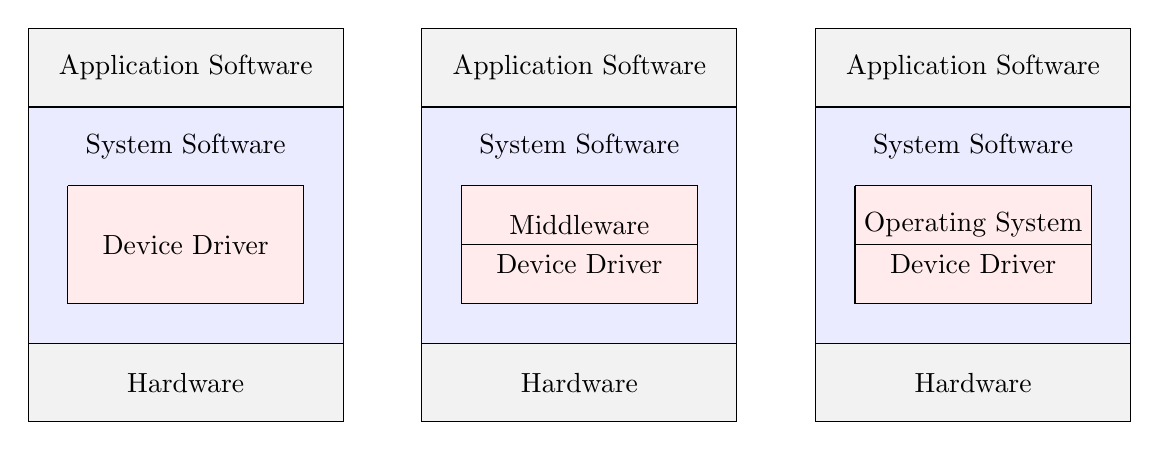
\begin{tikzpicture}
        \draw[fill=gray!10] (0,0) -- (4,0) -- (4,-5) -- (0,-5) -- (0,0);
        \draw[fill=blue!8] (0,-1) -- (4,-1) -- (4,-4) -- (0,-4) -- (0,-1);
        \draw[fill=red!8] (0.5,-2) -- (3.5,-2) -- (3.5,-3.5) -- (0.5,-3.5) -- (0.5,-2);

        \draw[fill=gray!10] (5,0) -- (9,0) -- (9,-5) -- (5,-5) -- (5,0);
        \draw[fill=blue!8] (5,-1) -- (9,-1) -- (9,-4) -- (5,-4) -- (5,-1);
        \draw[fill=red!8] (5.5,-2) -- (8.5,-2) -- (8.5,-3.5) -- (5.5,-3.5) -- (5.5,-2);
        \draw (5.5,-2.75) -- (8.5,-2.75);

        \draw[fill=gray!10] (10,0) -- (14,0) -- (14,-5) -- (10,-5) -- (10,0);
        \draw[fill=blue!8] (10,-1) -- (14,-1) -- (14,-4) -- (10,-4) -- (10,-1);
        \draw[fill=red!8] (10.5,-2) -- (13.5,-2) -- (13.5,-3.5) -- (10.5,-3.5) -- (10.5,-2);
        \draw (10.5,-2.75) -- (13.5,-2.75);

        \draw (2,-0.5) node[] {Application Software};
        \draw (2,-1.5) node[] {System Software};
        \draw (2,-2.75) node[] {Device Driver};
        \draw (2,-4.5) node[] {Hardware};
        
        \draw (7,-0.5) node[] {Application Software};
        \draw (7,-1.5) node[] {System Software};
        \draw (7,-2.5) node[] {Middleware};
        \draw (7,-3) node[] {Device Driver};
        \draw (7,-4.5) node[] {Hardware};
        
        \draw (12,-0.5) node[] {Application Software};
        \draw (12,-1.5) node[] {System Software};
        \draw (12,-2.5) node[] {Operating System};
        \draw (12,-3) node[] {Device Driver};
        \draw (12,-4.5) node[] {Hardware};
    \end{tikzpicture}
\end{center}
\caption{Embedded OSI system models}
\label{fig:embedded-osi}
\end{figure}


\textbf{NOTE}: Middleware is usually used on embedded systems with two or more applications, this
enables flexibility, security, portability, intercommunication and interoperability between
applications.

The advantages and disadvantages of different drivers is shown below:

\begin{itemize}
    \item OS-Supplied Drivers
    \begin{itemize}
        \item {No need to search for compatible drivers}
        \item \red{Only the most popular hardware is supported} 
    \end{itemize}

    \item Manufacturer Supplied Drivers
    \begin{itemize}
        \item {Availability reduces development time}
        \item \red{May not be optimal for a specific application} 
    \end{itemize}
    
    \item Direct Hardware Access
    \begin{itemize}
        \item {Very fast access}
        \item \red{May not take advantage of operating system features} 
    \end{itemize}
    
    \item Third Party Proprietary Driver
    \begin{itemize}
        \item {May add enhanced functionality}
        \item \red{Not avalible for all all operating systems or hardware} 
    \end{itemize}
    
    \item Roll Your Own Driver
    \begin{itemize}
        \item {May be highly optimised for the application}
        \item \red{May require significant development and testing time} 
    \end{itemize}
\end{itemize}

\subsection{Architecture Specific Driver}
Architecture specific drivers use a two layer structure, with the top layer being hardware
independent providing high level commands such as `\textit{uart\_write()}' these commands don't
perform low level operations and are therefore not MCU specific. The bottom layer is known as the
hardware abstraction layer (HAL) and is MCU specific as it directly interacts with hardware
registers.

\subsection{Controls in Drivers}
When designing drivers there are several considerations that need to be made, the first is regarding
errors, eg. `\textit{malloc()}' on failure returns \textit{NULL}, this indicates an error such as
insufficient memory. There are two conventional options for return types the first is, a small
integer eg. `-1' the second is a pointer. The advantages of using a small integer is that is is easy
to check and the disadvantage is that a mapping table is required. For pointers the advantage is
that it is faster as there is no table lookup and the disadvantage is that more memory is used.\\

\noindent Next the device needs a handle, used to specify the appropriate device.\\

\noindent Next is data passing, for this passing a pointer is typical\\

\noindent The most important factor however, is consistency for each of these components.

\subsection{Configuration Parameters}
There are two methods for passing configuration parameters to a device driver. The first is using a
static configuration, this is when the parameters are passed at compile time. This method is simple
how can become difficult to maintain. To create a static configuration macros, enums, header
definitions and conditional compilation can be used (compile options eg.
architecture). The second method is dynamic configuration, this is where the driver parameter
structures are passed into setup type functions at run-time, this model is used extensively for high
level languages. These configuration structures can be stored as an object library in an include
or object file.

\subsection{Performance Considerations}
Overall, the performance of the drivers is dependent on the hardware used. There are two main
operation type, the first is interrupt operation. This operation type is relatively low latency,
these interrupts can be software generated, external (based on pin change) or internal (DMA,
internal peripheral etc.). Using interrupts can result in components of the software being
non-deterministic as interrupts, especially ones on an external trigger can be unpredictable. The
second operation type is to use polling, this method is simple however can be very CPU intensive.
Polling is often integrated with RTOS.

\subsection{Multiple Devices}
To work with multiple devices the code must be `reentrant' this is when code returns to were it
started and doesn't move to a different one. This means that setting a global state then writing
will have issues whereas passing the value of a device to be written to/read from into the
read/write function.

